\documentclass[10pt]{article}
\usepackage[paper=letterpaper,
            marginparwidth=1.2in,     % Length of section titles
            marginparsep=.05in,       % Space between titles and text
            margin=1in]{geometry}
\usepackage{enumitem}
\usepackage{color,hyperref}
\definecolor{darkblue}{rgb}{0.0,0.0,0.6}
\hypersetup{colorlinks,breaklinks,
            linkcolor=darkblue,urlcolor=darkblue,
            anchorcolor=darkblue,citecolor=darkblue}
\usepackage{graphicx}

\begin{document}
\section{Team Members and Contact Information}
\begin{tabular}[width=6.5in]{l c r}
Name & E-mail & GitHub Username \\
Dr. Keshab K. Parhi & \href{mailto:parhi@umn.edu}{parhi@umn.edu} & \\
Mike Brown & \href{mailto:mjbrown.droid@gmail.com}{mjbrown.droid@gmail.com} & \href{http://www.github.com/mjbrown}{mjbrown} \\
\end{tabular}
\section{Project Summary}
From biomedical applications to robotics, there are several areas of electrical engineering research that use audio signals to do extraordinary things.  Several signal processing techniques, such as independent component analysis, principal component analysis, or beamforming, analyze several channels of audio simultaneously to extract useful information.  However, interfaces for recording more than two channels simultaneously are usually bulky and/or expensive.  The goal of this project is to create a small, inexpensive, and scalable audio recording device for use with a PC via USB.  The block diagram below shows the proposed audio interface.
\begin{figure}[!h]
\centering
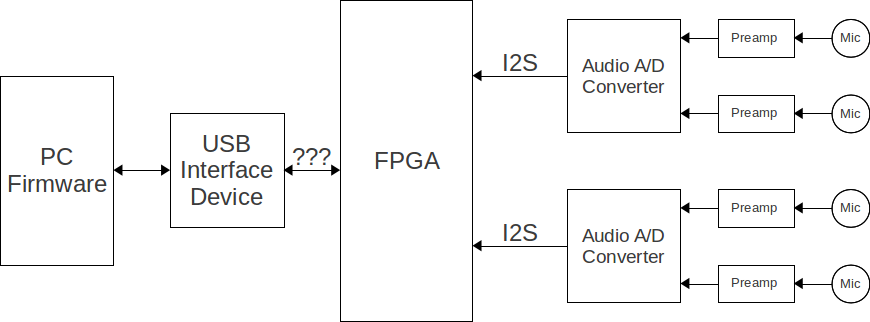
\includegraphics[width=6.5in]{block_diagram.png}
\caption{UMN Simultaneous Audio Recording Interface Block Diagram}
\label{fig:block_diagram}
\end{figure}
\section{Customer Requirements}
The following requirements must be met for this device to perform the functionality desired:
\begin{itemize}
\item
Minimum 16-bit resolution pulse code modulated (PCM) data.
\item
Minimum 16kHz sampling frequency.
\item
Minimum \emph{FOUR} channels of simultaneous recording.
\item
Usable for researchers with zero knowledge of microcontrollers or FPGA details.
\end{itemize}
The following are highly desirable qualities, but are not absolutely essential to the success of the project:
\begin{itemize}
\item
Reconfigurable resolution from 8-bit to 24-bit.
\item
Reconfigurable sampling frequency from 1kHz to 96kHz.
\item
Reconfigurable number of input channels.
\item
Minimum profile, stackable/mountable, and USB powered for ultimate portability.
\end{itemize}
\section{Design Challenges}
\subsection{Data Throughput}
The primary challenge for this project is handling the enormous amounts of data throughput required from all communications interfaces.  For example, a single channel of 96kHz audio with 24 bits of resolution requires a minimum of 2.3 megabits of data throughput for real-time data processing.  An FPGA can handle this volume of data, and provides additional advantages:
\begin{itemize}
\item
Audio A/D converters such as \href{http://www.nxp.com/documents/data\_sheet/UDA1361TS.pdf}{NXP's UDA1361TS} require a system clock at 256 times the sampling frequency.  FPGAs can produce such a clock very easily.
\item
The same A/D converter uses the I2S digital communications protocol.  An FPGA can be configured as a master to drive the I2S clock and channel select lines very precisely.
\item
The A/D converter produces 24-bit resolution data.  The FPGA can be configured to truncate or round the data to 16-bits with little difficulty.
\item
Simply running the A/D converter at a lower sampling frequency will introduce aliasing to the input data, severely degrading signal quality.  If an analog filter is inserted after the \href{http://datasheets.maxim-ic.com/en/ds/MAX9812-MAX9813L.pdf}{microphone preamp} to remove high frequency components, then the hardware can never be used for higher sampling rates.  An FPGA can collect the data at a high sampling frequency and use digital signal processing (DSP) to downsample the data without quality loss.  If 10-20 input channels are used, a microcontroller would have insufficient processing power to handle all of the DSP calculations simultaneously.
\item
Future applications may implement other operations into the FPGA.  A spacial FFT could be used for coarse direction finding applications.  Adaptive beamformers could be implemented for finer direction finding.  Feature extraction could be performed by the FPGA for a machine learning application.  Professor Parhi's group are experts in digital signal processing architectures, and a reconfigurable hardware platform for audio processing will be a powerful tool for their future research.
\end{itemize}
Creating a static design which incorporates a specific number of microphones, a specific sampling frequency, and a specific resolution would be short-sighted and limited in its usefulness.  \href{http://introlab.gel.usherbrooke.ca/mediawiki-introlab/index.php/8SoundsUSB}{An inflexible multi-channel audio capture interface already exists}.
\subsection{Software Collaboration}
With 6 team members and a great deal of software development required, it will be a learning experience in software collaboration for everyone involved.  All team members should become familiar with the revision control software Git.  \href{http://www.vogella.de/articles/Git/article.html}{This tutorial} will take 20-30 minutes to walk through, and is an excellent start.  Create an account on GitHub, the repository has already been created at \href{http://github.com/mjbrown/umn\_simaudio}{https://github.com/mjbrown/umn\_simaudio}.
\subsection{Hardware Development}
The smallest Spartan-3E FPGAs have 100+ pins, and layout/soldering of such a complex device is probably beyond the capabilities of most of the group.  First and foremost, a PCB layout with an A/D converter, microphone preamp, microphone, and supporting components needs to be designed and prototyped.  \href{http://www.nxp.com/documents/data_sheet/UDA1361TS.pdf}{This A/D Converter} and \href{http://datasheets.maxim-ic.com/en/ds/MAX9812-MAX9813L.pdf}{this microphone preamp} will meet the requirements of this project, but the group is welcome to find alternatives.  Ten \href{http://www.digilentinc.com/Products/Detail.cfm?Prod=BASYS2}{Basys-2 Development Boards} are available, with upgraded FPGAs (250k gates instead of 100k).  RS232 conversion Pmods are also available so that data can be brought to the PC during early development.  The Basys-2 development boards have USB capability built-in, but most sample code is in VHDL so the exact capabilities are unknown.
\par
An alternative solution would be to hack an \href{http://dangerousprototypes.com/docs/Open_Bench_Logic_Sniffer}{Open Bench Logic Sniffer}.  This device has a PIC18F26J50 for USB and the same 250k gate Spartan-3E FPGA that is in our Basys-2 development boards.  The FPGA has 32+ pins of I/O available which could connect to 20+ A/D converters.  The design is open source, so all design schematics, layout, and source code are freely available.
\end{document}

